\chapter{拉普拉斯变换}

傅里叶变换将信号从时域变换为频域,但是没有考虑信号的增益,或者说假设信号不变。
但真实系统一定存在信号的增益,而且通常衰减是以指数形式。
拉普拉斯变换通过引入实指数描述信号的增益,使得其能够描述系统。

其次,因果LTI系统输入输出关系一般使用微分方程描述,而拉普拉斯变换可以将微分方程转变为代数关系,称为传递函数。
传递函数将时域的微分和积分关系转化为复频域的代数关系,使得计算分析变得简单。

本章要点:
\begin{itemize}
    \item 拉普拉斯变换。
\end{itemize}

\newpage
\section{拉普拉斯变换}

本节介绍拉普拉斯变换。

本节要点:
\begin{itemize}
    \item 掌握拉普拉斯变换的定义;
    \item 了解拉普拉斯变换的性质。
\end{itemize}

%============================================================
\subsection{拉普拉斯变换的概念}

\begin{definition}[拉普拉斯变换]
若信号$x\left( t \right) $满足积分$\int_{-\infty}^{+\infty}{x\left( t \right) e^{-st}dt}$收敛,其中$s=\sigma +i\omega $为复数,则称该积分为{\bf $x\left( t \right) $的拉普拉斯变换}(Laplace Transform,LT),记为$X\left( s \right) $,即:
\[
X\left( s \right) =\int_{-\infty}^{+\infty}{x\left( t \right) e^{-st}dt}
\]
又称为{\bf 双边拉普拉斯变换}。
称满足积分收敛条件的$s$的定义域为{\bf 拉普拉斯变换的收敛域}。
同时将
\[
X\left( s \right) =\int_0^{+\infty}{x\left( t \right) e^{-st}dt}
\]
称为{\bf 单边拉普拉斯变换}。
若无特别指明,本笔记LT均指单边拉普拉斯变换。
相应地称
\[
x\left( t \right) =\frac{1}{2\pi i}\int_{c-i\infty}^{c+i\infty}{X\left( s \right) e^{st}ds}
\]
为{\bf 拉普拉斯逆变换},其中$c$为任意实数,且需满足$s=c+i\omega $始终在LT的收敛域内。
$x\left( t \right) $及其拉普拉斯变换形式通常记为:
\[
x\left( t \right) \overset{\mathscr{L}}{\leftrightarrow}X\left( s \right)
\]
\end{definition}

LT是一个自变量为复数的复函数。
LT相较于FT加入了一个收敛因子$e^{-\sigma}$,收敛域根据具体信号而定,不同的信号有不同的收敛域。
可以认为LT是广义的FT,只要是信号的LT收敛域包括$\sigma =0$,就有FT。
LT的优势在于对一个LTI系统,可以将其微分方程和初始条件一并变换成一个代数方程。

至此,我们对于信号或系统有了3个可供描述的空间:1)以微分方程和卷积为代表的时域;2)用FT得到的频域;3)用LT得到的s域。

~

\begin{example}
求信号$x\left( t \right) =e^{-bt}u\left( t \right) ,t\geqslant 0$的LT,其中$b\in \mathbb{R} $。
\end{example}

当$b+\sigma <0$时,有$\underset{t\rightarrow +\infty}\lim e^{-\left( b+s \right) t}=0$,则:
\[
X\left( s \right) =\frac{1}{b+s}
\]
收敛域是$\mathrm{Rs}\left[ s \right] >-b$。
特别地,当$b<0$时,信号有FT:
\[
X\left( \omega \right) =\frac{1}{b+i\omega}
\]

%============================================================
\subsection{拉普拉斯变换的性质}

{\bf 线性性}(由于积分的线性性,不证自明)
\[
ax\left( t \right) +by\left( t \right) \leftrightarrow aX\left( s \right) +bX\left( s \right)
\]

{\bf 时延性、频移性}(积分变量做一个变换即可证明)
\begin{align*}
&x\left( t-t_1 \right) u\left( t-t_1 \right) \leftrightarrow X\left( s \right) e^{-st_1} \qquad t_1>0 \\
&e^{s_1t}\cdot x\left( t \right) \leftrightarrow X\left( s-s_1 \right) \qquad s_1\in \mathbb{C}
\end{align*}

LT中的时移必须时延迟,即时间右移,左移是不存在的,因为LT的单边性使得左移后函数削掉了一部分。

{\bf 时展性}(积分变量做一个变换即可证明)
\[
x\left( at \right) \leftrightarrow \frac{1}{a}X\left( \frac{s}{a} \right) \qquad a>0
\]

LT中没有类似FT中的时间轴反转。

{\bf 三角律}(频移性结合欧拉公式即可证明)
\begin{align*}
&x\left( t \right) \cos \omega _1t\leftrightarrow \frac{1}{2}\left[ X\left( s+i\omega _1 \right) +X\left( s-i\omega _1 \right) \right] \\
&x\left( t \right) \sin \omega _1t\leftrightarrow \frac{i}{2}\left[ X\left( s+i\omega _1 \right) -X\left( s-i\omega _1 \right) \right]
\end{align*}

{\bf 时域的微分和积分}
\begin{align*}
&\frac{d^nx\left( t \right)}{dt^n}\leftrightarrow s^n\cdot X\left( s \right) -\sum_{i=1}^n{s^{n-i}\frac{d^{i-1}x\left( 0^- \right)}{dt^{i-1}}} \\
&\int_{-\infty}^t{x\left( \tau \right) d\tau}\leftrightarrow \frac{1}{s}\cdot X\left( s \right)
\end{align*}
特别地有:
\begin{align*}
&x'\left( t \right) \leftrightarrow s\cdot X\left( s \right) -x\left( 0^- \right) \\
&x''\left( t \right) \leftrightarrow s^2\cdot X\left( s \right) -s\cdot x\left( 0^- \right) -x'\left( 0^- \right)
\end{align*}

{\bf 频域的微分}
\[
t^n\cdot x\left( t \right) \leftrightarrow \left( -1 \right) ^n\frac{d^nX\left( s \right)}{ds^n}
\]

{\bf 卷积性}
\[
x\left( t \right) \ast y\left( t \right) \leftrightarrow X\left( s \right) Y\left( s \right)
\]

{\bf 初值定理}:已知信号$x\left( t \right) \leftrightarrow X\left( s \right) $,则其n阶导数的初值为:
\[
\left. \frac{d^nx\left( t \right)}{dt^n} \right|_{t=0^+}=\underset{s\rightarrow \infty}\lim \left[ s^{n+1}\cdot X\left( s \right) -\sum_{i=1}^n{s^{n+1-i}\frac{d^{i-1}x\left( 0^+ \right)}{dt^{i-1}}} \right]
\]
特别地有:
\begin{align*}
&x\left( 0 \right) =\underset{s\rightarrow \infty}\lim \left[ s\cdot X\left( s \right) \right] \\
&x'\left( 0 \right) =\underset{s\rightarrow \infty}\lim \left[ s^2\cdot X\left( s \right) -s\cdot x\left( 0 \right) \right]
\end{align*}

初值定理使得我们在已知$X\left( s \right) $而未知$x\left( t \right) $的情况,无需通过iLT直接求得$x\left( 0 \right) $。
其次,由于LT的单边性,我们得到是$x\left( 0 \right) $或$x\left( 0^+ \right) $,不是$x\left( 0^- \right) $!

{\bf 终值定理}:已知信号$x\left( t \right) $的LT为$X\left( s \right) $,如果$x\left( t \right) $存在,则有:
\[
\underset{t\rightarrow +\infty}\lim x\left( t \right) =\underset{s\rightarrow 0}\lim \left[ s\cdot X\left( s \right) \right]
\]

\begin{tcolorbox}
注意,LT没有FT中的“Duality”和“Parsevel定理”。
\end{tcolorbox}






\newpage
\section{拉普拉斯逆变换}

本节介绍拉普拉斯逆变换。
由于从定义上iLT非常难解,而实际中多数LT的形式是有理式,这里只针对有理式的形式给出留数解。

本节要点:
\begin{itemize}
    \item 了解拉普拉斯逆变换的留数解;
    \item 了解极点类型对逆变换的影响;
    \item 掌握通过极点类型判断逆变换形状。
\end{itemize}

%============================================================
\subsection{有理式、零点和极点}

\begin{definition}
如果信号$x\left( t \right) $的LT可以表达为一个有理式:
\[
X\left( s \right) =\frac{B\left( s \right)}{A\left( s \right)}=\frac{b_ms^m+\cdots +b_1s+b_0}{a_ns^n+\cdots +a_1s+a_0}
\]
\begin{itemize}
    \item $b_i,a_i\in \mathbb{R} $:实系数,且$b_m,a_n\ne 0$;
    \item $m,n\in \mathbb{Z} ^+$:正整数,特别地称{\bf $n$为$X\left( s \right) $的阶数};
    \item $B\left( s \right) ,A\left( s \right) $:{\bf 分子多项式}(numerator polunomial)和{\bf 分母多项式}(denominator polynomial),且它们无公因式。
\end{itemize}
将$A\left( s \right) $化成多项式:
\[
A\left( s \right) =a_n\prod_{i=1}^n{\left( s-p_i \right)}
\]
其中$p_i\in \mathbb{C} $为$A\left( s \right) =0$的根,称为{\bf $A\left( s \right) $的零点}。
如果某一个零点是复数,则其共轭复数也是零点,也即复数零点成共轭对出现。
相应的LT可写为:
\[
X\left( s \right) =\frac{B\left( s \right)}{a_n\prod_{i=1}^n{\left( s-p_i \right)}}
\]
此时,$p_i$也称为{\bf $X\left( s \right) $的极点}。
$A\left( s \right) =0$也可称为{\bf 系统的特征方程},$p_i$也称{\bf 系统的特征根}。
\end{definition}

$p_i$对于$A\left( s \right) $称为零点,对于$X\left( s \right) $称为极点,对于系统称为特征根。
所有项中,我们最关心$p_i$,它决定了系统的稳定性。

%============================================================
\subsection{Python应用——numpy.roots函数}

Numpy中的roots函数求解多项式的根。
\begin{figure}[ht]
\centering
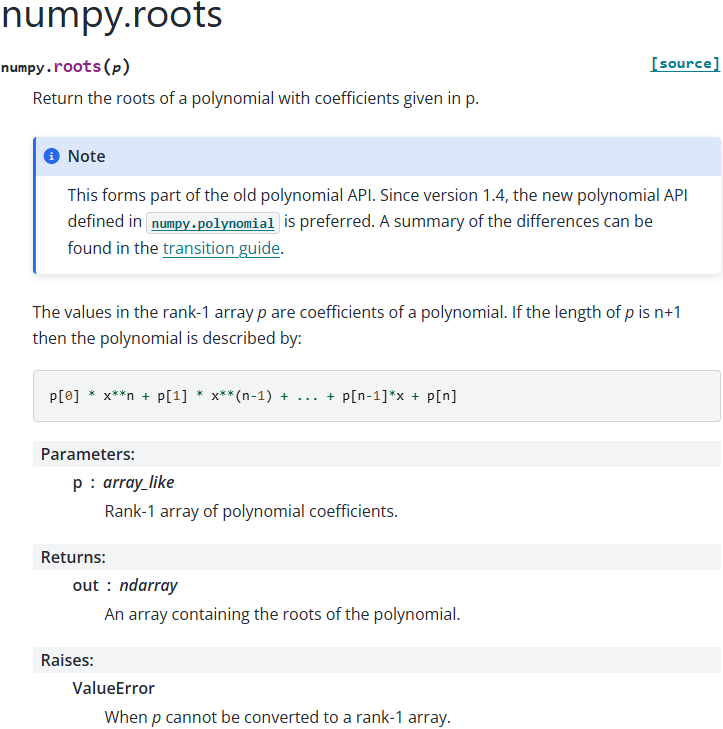
\includegraphics[width=10cm]{7.2.2-1.png}
\end{figure}

~

\begin{example}
如有多项式$A\left( s \right) =s^3+4s^2+6s+4$,求根。
\end{example}

\begin{python}
>>> import numpy as np
>>> p = np.roots([1, 4, 6, 4])
>>> p
array([-2.+0.j, -1.+1.j, -1.-1.j])
\end{python}

%============================================================
\subsection{iLT的留数解——单极点}

设LT变换:
\[
X\left( s \right) =\frac{B\left( s \right)}{A\left( s \right)} \qquad m<n
\]
若有{\bf 单极点}(distinct pole,即$p_i\ne p_j$),用留数方法求解拉普拉斯逆变换,步骤如下:
\begin{enumerate}
    \item 首先求得极点$p_i$的值,于是LT可化为极点的和式:
    \[
    X\left( s \right) =\sum_{i=1}^n{\frac{c_i}{s-p_i}}=\frac{c_1}{s-p_1}+\frac{c_2}{s-p_2}+\cdots +\frac{c_n}{s-p_n}
    \]
    \item 求得留数$c_i$:
    \[
    c_i=\left. \left[ \left( s-p_i \right) X\left( s \right) \right] \right|_{s=p_i}
    \]
    \item 由于LT的线性性,可得逆变换:
    \[
    x\left( t \right) =\sum_{i=1}^n{c_ie^{p_it}}=c_1e^{p_1t}+c_2e^{p_2t}+\cdots +c_ne^{p_nt} \qquad t\geqslant 0
    \]
\end{enumerate}
注意:
\begin{itemize}
    \item 如果单极点是实数,则留数也是实数,iLT结果的对应项是$ce^{p_it}$,表示时域呈指数发散或收敛;
    \item 如果单极点有复数,则必以共轭对$p_i,\bar{p}_i=\sigma \pm i\omega $的形式出现,对应留数也有共轭对$c_i,\bar{c}_i$,此时,时域中的共轭对必能合并为实数项$c_ie^{p_it}+\bar{c}_ie^{\bar{p}_it}=2\left| c_i \right|e^{\sigma t}\cos \left( \omega t+\angle c_i \right) $,表示以指数包络振荡;
    \item 如果单极点是纯虚数$\sigma =0$,也是共轭对$p_i,\bar{p}_i=\pm i\omega $,iLT结果项为$2\left| c_i \right|\cos \left( \omega t+\angle c_i \right) $,表示时域稳定震荡。
\end{itemize}

\begin{tcolorbox}
可结合微积分中的二阶微分方程理解iLT的收敛项和振荡项。
\end{tcolorbox}

%============================================================
\subsection{iLT的留数解——重复极点}

若拉普拉斯变换如下:
\[
X\left( s \right) =\frac{c_1}{s-p_1}+\frac{c_2}{\left( s-p_1 \right) ^2}+\frac{c_3}{\left( s-p_1 \right) ^3}+\cdots +\frac{c_r}{\left( s-p_1 \right) ^r}+\cdots
\]
极点$p_1$有$r$次重复,相应的留数:
\[
c_i=\frac{1}{\left( r-i \right) !}\cdot \left. \left[ \frac{d^{r-i}}{ds^{r-i}}\left[ \left( s-p_1 \right) ^rX\left( s \right) \right] \right] \right|_{s=p_1} \qquad i=1,2,\cdots ,r
\]
即:
\begin{align*}
&c_1=\frac{1}{\left( r-1 \right) !}\cdot \left. \left[ \frac{d^{r-1}}{ds^{r-1}}\left[ \left( s-p_1 \right) ^rX\left( s \right) \right] \right] \right|_{s=p_1} \\
&c_2=\frac{1}{\left( r-2 \right) !}\cdot \left. \left[ \frac{d^{r-2}}{ds^{r-2}}\left[ \left( s-p_1 \right) ^rX\left( s \right) \right] \right] \right|_{s=p_1} \\
&\vdots \\
&c_{r-2}=\frac{1}{2!}\cdot \left. \left[ \frac{d^2}{ds^2}\left[ \left( s-p_1 \right) ^rX\left( s \right) \right] \right] \right|_{s=p_1} \\
&c_{r-1}=\left. \left[ \frac{d}{ds}\left[ \left( s-p_1 \right) ^rX\left( s \right) \right] \right] \right|_{s=p_1} \\
&c_r=\left. \left[ \left( s-p_1 \right) ^rX\left( s \right) \right] \right|_{s=p_1}
\end{align*}
再根据LT性质$\frac{t^{n-1}}{\left( n-1 \right) !}e^{-at}\leftrightarrow \frac{1}{\left( s+a \right) ^n}$即可得到iLT的对应项。
这种情况下,信号会包含$t$的次方的多项式。

%============================================================
\subsection{iLT的留数解——总结}

极点类型及数量决定了时域的形状(收敛、发散、振荡),分子多项式$B\left( s \right) $不影响的形状,只影响留数$c_i$的值。
\begin{table}[h]
\centering
% \caption{表头}
\begin{tabular}{ccc}
    \toprule
    极点类型 & 时域包含项 & 物理意义\\
    \midrule
    实数单极点 & $ce^{pt}$ & 增益项\\
    复数单极点 & $2\left| c \right|e^{\sigma t}\cos \left( \omega t+\angle c \right) $ & 振荡项\\
    重复点 & $c_1e^{pt}+c_2te^{pt}+c_3t^2e^{pt}+\cdots $ & \\
    \bottomrule
\end{tabular}
\end{table}

%============================================================
\subsection{Python应用——scipy.signal.residue函数}

Python的Scipy库的signal模块有residue()函数专用于求解留数。
\begin{figure}[h]
\centering
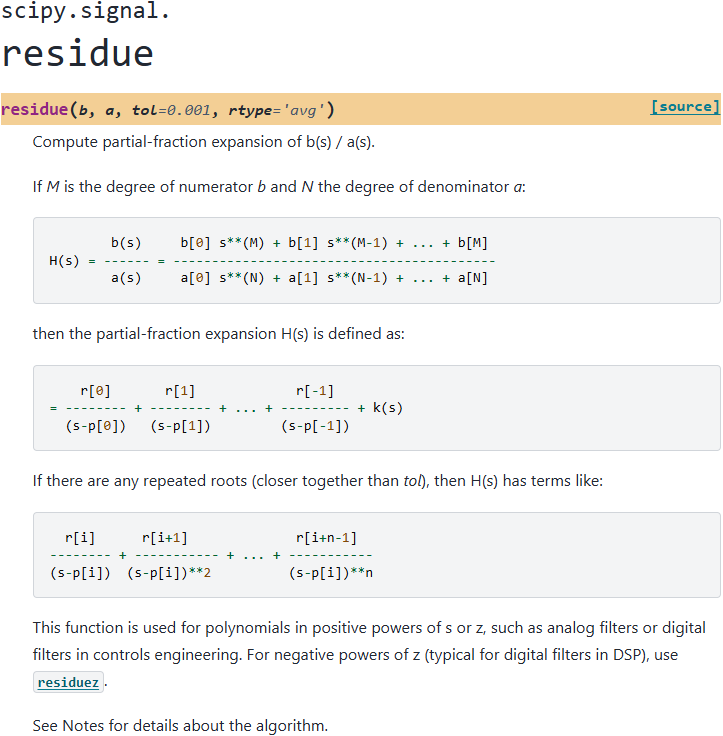
\includegraphics[width=10cm]{7.2.6-1-1.png}
\end{figure}
\begin{figure}[ht]
\centering
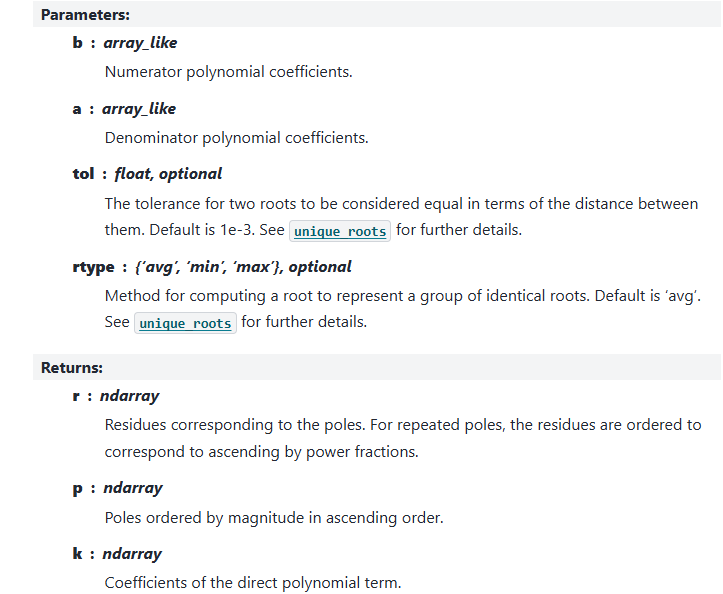
\includegraphics[width=10cm]{7.2.6-1-2.png}
\end{figure}

~

~

~

~

\begin{example}
如信号$x\left( t \right) $的拉普拉斯变换$X\left( s \right) =\frac{s+2}{s^3+4s^2+3s}$,求$x\left( t \right) $。
\end{example}

\begin{python}
import numpy as np
from scipy import signal

import fractions
np.set_printoptions(formatter={'all':lambda x: str(fractions.Fraction(x).limit_denominator())})

b = [1,2]
a = [1,4,3,0]
r,p,k = signal.residue(b, a)

=====output=====
b = [2/3 -1/2 -1/6]
p = [0 -1 -3]
k = []
\end{python}

注意,我们导入fractions模块,并设置np的值都以分数形式打印。
得到信号:
\[
x\left( t \right) =\frac{2}{3}+\left( -\frac{1}{2} \right) e^{-t}+\left( -\frac{1}{6} \right) e^{-3t} \qquad t\geqslant 0
\]
由于极点都是实数解,且都小于0,所以$x\left( t \right) $最终是指数衰减。

~

\begin{example}
如信号$x\left( t \right) $的拉普拉斯变换$X\left( s \right) =\frac{s^2-2s+1}{s^3+3s^2+4s+2}$,求$x\left( t \right) $。
\end{example}

\begin{python}
import numpy as np
from scipy import signal

b = [1,-2,1]
a = [1,3,4,2]
r,p,k = signal.residue(b, a)

=====output=====
r = [ 4. +0.j -1.5+2.j -1.5-2.j]
p = [-1.+0.j -1.+1.j -1.-1.j]
k = []
\end{python}

得到一个实数极点和一对共轭对极点:
\[
\begin{cases}
	p_1=-1\\
	c_1=4\\
\end{cases} \qquad \begin{cases}
	p_2,\bar{p}_2=1\pm i\\
	c_2,\bar{c}_2=-\frac{2}{3}\pm 2i\\
\end{cases}
\]
最终得到信号:
\begin{align*}
x\left( t \right) &=4e^{-t}+c_2e^{p_2t}+\bar{c}_2e^{\bar{p}_2t}=4e^{-t}+2\left| c_2 \right|e^t\cos \left( t+\angle c_2 \right) \\
&=4e^{-t}+5e^{-t}\cos \left( t+126.87^{\circ} \right)
\end{align*}






\newpage
\section{拉普拉斯变换应用——求解微分方程}

由于拉普拉斯变换的时域的微分性质,LT特别适用于求解微分方程,这给求解系统输出带来方便。

本节要点:
\begin{itemize}
    \item 掌握通过LT求解系统微分方程。
\end{itemize}

%============================================================
\subsection{求解系统微分方程}

用LT求解微分方程步骤:
\begin{enumerate}
    \item 写出系统微分方程。
    \item 两边分别求LT,得到对应的拉普拉斯变换形式。
    \item 求信号的LT,带入得到输出的拉普拉斯变换。
    \item 求iLT,得到输出。
\end{enumerate}

~

若LTI系统有一阶微分方程
\[
\frac{dy\left( t \right)}{dt}+Py\left( t \right) =Qx\left( t \right)
\]
两边LT,得到:
\begin{align*}
&sY\left( s \right) -y\left( 0^- \right) +PY\left( s \right) =QX\left( s \right) \\
&Y\left( s \right) =\frac{1}{s+P}y\left( 0^- \right) +\frac{Q}{s+P}X\left( s \right)
\end{align*}
称为{\bf 系统的复频域表达式}。
输出由初始能量和对输入的响应组成。
特别地,当系统无初始能量时($y\left( 0^- \right) =0$),有:
\[
Y\left( s \right) =\frac{Q}{s+P}X\left( s \right)
\]
令$H\left( s \right) =\frac{Q}{s+P}$,称为{\bf 系统的传递函数}(transfer function)。

若LTI系统有二阶微分方程
\[
\frac{d^2y\left( t \right)}{dt^2}+P_1\frac{dy\left( t \right)}{dt}+P_0y\left( t \right) =Q_1\frac{dx\left( t \right)}{dt}+Q_0x\left( t \right)
\]
两边LT,且由于$x\left( t \right) =0,t<0$,得到:
\[
Y\left( s \right) =\frac{sy\left( 0^- \right) +y'\left( 0^- \right) +P_1y\left( 0^- \right)}{s^2+P_1s+P_0}+\frac{Q_1sX\left( s \right) +Q_0X\left( s \right)}{s^2+P_1s+P_0}
\]
特别地,系统无初始储能时有
\[
Y\left( s \right) =\frac{Q_1s+Q_0}{s^2+P_1s+P_0}X\left( s \right)
\]
称$H\left( s \right) =\frac{Q_1s+Q_0}{s^2+P_1s+P_0}$为{\bf 二阶系统的传递函数}。

更一般地,若LTI系统是n阶微分方程
\[
y^{\left( n \right)}\left( t \right) +\sum_{i=0}^{n-1}{A_iy^{\left( i \right)}\left( t \right)}=\sum_{i=0}^m{B_ix^{\left( i \right)}\left( t \right)}
\]
系统无初始储能时,传递函数为
\[
H\left( s \right) =\frac{B_ms^m+\cdots +B_1s+B_0}{s^n+A_{n-1}s^{n-1}+\cdots +A_1s+A_0}
\]

%============================================================
\subsection{例}

\begin{example}
还是以RC电路为例,假设电容有初始储能$y\left( 0^- \right) $,输入为$x\left( t \right) =u\left( t \right) $,分析输出。
\begin{figure}[h]
\centering
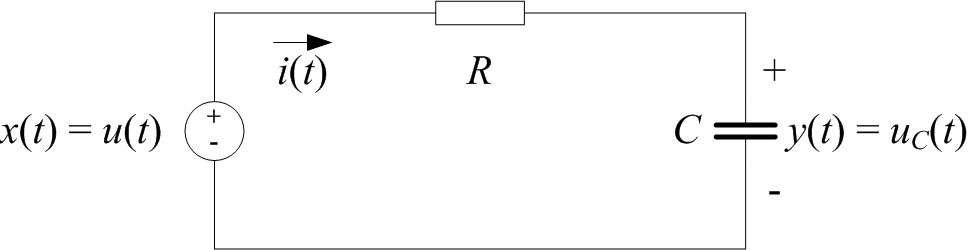
\includegraphics[height=2cm]{1.5.1-1.png}
\end{figure}
\end{example}

系统的微分方程为:
\[
\frac{dy\left( t \right)}{dt}+\frac{1}{RC}y\left( t \right) =\frac{1}{RC}x\left( t \right)
\]
复频域表达式:
\begin{align*}
Y\left( s \right) &=\frac{y\left( 0^- \right)}{s+\left( 1/RC \right)}+\frac{\left( 1/RC \right)}{s+\left( 1/RC \right)}X\left( s \right) \\
&=\frac{y\left( 0^- \right)}{s+\left( 1/RC \right)}+\frac{\left( 1/RC \right)}{s+\left( 1/RC \right)}\cdot \frac{1}{s} \\
&=\frac{y\left( 0^- \right)}{s+\left( 1/RC \right)}+\frac{1}{s}-\frac{1}{s+\left( 1/RC \right)}
\end{align*}
iLT后得到:
\[
y\left( t \right) =y\left( 0^- \right) e^{-\left( 1/RC \right) t}+1-e^{-\left( 1/RC \right) t}
\]
若系统无初始储能,则$y\left( t \right) =1-e^{-\left( 1/RC \right) t}$。






\newpage
\section{本章小结}

本章介绍了拉普拉斯变换。

拉普拉斯变换的工程意义在于传递函数。
传递函数可以非常直观的建立和分析系统。
通常,我们只需要通过系统组件的LT形式直接构建系统的传递函数,而不用通过微分方程求解。









